\chapter{Theoretische Grundlagen}\label{sec:basics}

In diesem Kapitel werden die für den Forschungshintergrund und die Entwicklung des Prototyps wichtigen theoretischen Grundlagen beschrieben.m
Zunächst werden verschiedene Theorien zu Kommunikationsmodellen vorgestellt, die dem Modell dieser Anwendung zugrunde liegen.
Im Anschluss daran werden die in der Ludologie beschriebenen Akteurstypen vorgestellt, die sich in den Teilnehmenden dieser Masterarbeitsstudie wiederspiegeln.
Allgemein ist bekannt, dass Video- und Computerspiele drei verschiedene Modi haben können: Singleplayer, Multiplayer und Mischformen. Da im Rahmen dieser Studie ein Multiplayer-Spiel konzipiert und umgesetzt wurde, werden im weiteren Verlauf verschiedene Kategorien von Multiplayer-Spielen vorgestellt. Außerdem werden die damit einhergehenden Netzwerkinfrastrukturen dargestellt, die für die aktuelle sowie eine potenzielle zukünftige Entwicklung relevant sind.

\section{Kommunikationsmodelle}
[Literatur suchen]
% In der Kommunikationswissenschaft wird die Kommunikation in 2 Arten unterteilt, die Massen- und Individualkommunikation.
[hier spielen dann auch die parameter ne Rolle, die kommunikation anspricht oder enthält]
\subsection{Nach Schulz von Thun}
\subsection{Nach Wazlawik}
\subsection{Nach Rogers}

% [Könnte besser in die Einleitung passen
% \section{Spiele als soziales Medium}
% \cite{depping_trust_2016}
% \cite{gerling_designing_2014}
% \cite{ducheneaut_alone_2006}
% ]

\section{Spielertypen}
Die Kommunikationswissenschaft umfasst zwar den Schwerpunkt dieser Arbeit, jedoch wurden auch ludologische Aspekte berücksichtigt. Dabei handelt es sich um die wissenschaftliche Auseinandersettung mit dem Spiel selbst (vgl. \cite{ludologie_spielforschung_nodate}). 

Im Hinblick auf die Konzeption und Entwicklung eines Spiels ist es wichtig, die Eigenschaften des Spielsystems so zu gestalten, dass sie Begeisterung und Engagement bei der gewünschten Zielgruppe hervorrufen. Aus diesem Grund muss zunächst die Zielgruppe in verschiedene Typen eingeteilt werden. Die  Ludologie unterscheidet hierfür verschiedene Spielertypen. Zwar ist nicht jeder Mensch ein \say{Spielertyp}, dennoch kann er grundsätzlich durch unterschiedliche Spielelemente angesprochen werden (vgl. \cite{ludologie_spielertypen_nodate}).

\subsection{Nach Bartle}
1996 beschäftigte sich Richard Bartle mit der Frage, welche Spielertypen in der Ludologie unterschieden werden können. Dabei ging es zunächst um Klassifizierungen von Ansätzen, die beim Spielen von sogenannten \ac{MUD}s existieren (vgl. \cite{bartle_hearts_1996}). Diese Klassifizierungen werden noch heute für die Einteilung in Spielertypen herangezogen.

Bartle unterscheidet bei der Einteilung der Spielertypen zwei grundlegende Interessen (vgl. Abbildung \ref{fig:bartle-muds}):

\begin{figure}[ht]
\centering
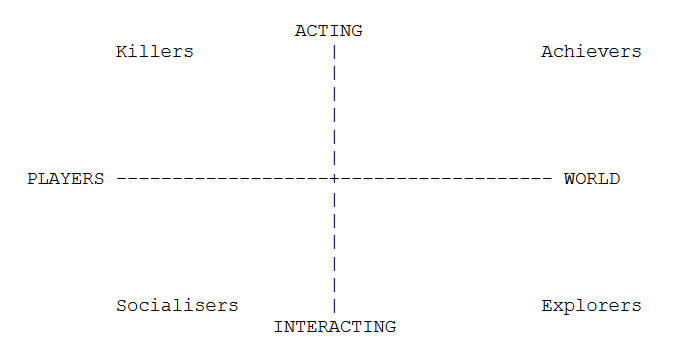
\includegraphics[width=1\linewidth]{content/pictures/basic_interests.PNG}
\caption{Interessen Graph nach Bartle (Quelle: \cite{bartle_hearts_1996})}
\label{fig:bartle-muds}
\end{figure}

Auf der X-Achse wird unterschieden, ob Spieler ihre Spielerfahrung über das Verhalten der anderen Mitspieler (Players) oder über die Spielwelt (World) definieren. Entlang der Y-Achse wird unterschieden, ob Spieler eher selbst aktiv Einfluss auf die Spielwelt nehemen möchten (Acting) oder ob sie in eine tiefere Interaktion mit ihr eingehen wollen (Interacting).

Die daraus resultierenden Typen sind:
\paragraph{Achiever}
Sie sind daran interessiert, auf die Spielewelt einzuwirken und alle ihnen gestellten Aufgaben mit Erfolg zu absolvieren. Ihr Status im Spiel ist ihnen wichtig - ebenso wie die Effizienz, mit der sie Fortschritte erzielen.

\paragraph{Explorer}
Sie wollen vom Spiel überrascht werden und intensiv mit der Spielwelt interagieren. Die virtuelle Welt löst ein Gefühl des Staunens aus, nach dem sie aktiv suchen. Sie sind stolz auf das Wissen, das sie im Spiel sammeln. Das erlangte Wissen  möchten sie gerne an neue Spieler weitergeben.

\paragraph{Socialiser}
Sie wollen mit anderen Spielern interagieren, meist über Gespräche, aber auch durch ungewöhnliche oder kreative Verhaltensweisen. Andere Menschen kennenzulernen und mehr über sie zu erfahren, ist für sie wertvoller als für andere. Die Spielwelt dient dabei lediglich als Kulisse - entscheidend sind für sie die Begegnungen mit anderen Charaktere. Sie sind stolz auf Freundschaften, ihre Kontakte und ihren Einfluss.

\paragraph{Killer}
Sie sind daran interessiert, auf andere Spiele einzuwirken und mit ihnen zu interagieren - häufig ohne deren Einverständnis. Sie wollen ihre Überlegenheit gegenüber anderen Menschen demonstrieren und sind stolz auf ihren Ruf sowie ihre oft geübten Kampffähigkeiten.

(vgl. \cite{bartle_hearts_1996}).

\subsection{Erweiterte Einteilungen}
Bartle ist nicht der Einzige, der sich mit Spielertypen auseinandergesetzt hat. Seine Forschung bildet jedoch ein grundlegendes Fundament, das in der weiteren wissenschaftlichen Auseinandersetzung intensive Diskussionen innerhalb der Forschungs- und Game-Design-Community ausgelöst hat. 
\begin{quote}
    \textit{
        \enquote{Player types are not a defined concept and any categorization of players or users needs to occur within the context of a particular application or domain. Play-personas are suggested as a useful tool that can be used to put player type research into practice as part of the design process of gamified systems.}
    } 
    (\cite{dixon_player_nodate})
\end{quote}

\paragraph{Dixon} 
stellt Spieler-Personae vor, die analog zum \ac{UCD}-Prozess eingesetzt werden können. Dadurch muss im Designprozess nicht strikt zwischen Motivation, Verhalten und Vorlieben unterschieden werden, da Personae als ausführliche, erzählerische Darstellung gedacht sind (vgl. \cite{dixon_player_nodate}).

\paragraph{Bateman und Boon}
entwickelten in ihrer 2005 erschienenen Studie zur Bestimmung des ersten Modells des Demographic Game Design (DGD1) vier Spielstile, die sie durch die Einbeziehung des \ac{MBTI} ableiteten (vgl. \cite{noauthor_mbti_nodate}; \cite{bateman_21st_2005}).
% Conquerer (Eroberer), Manager, Wanderer (Wanderer) und Participant (Teilnehmer) waren dabei die vier Spielstile.
Die vier Spielstile lauteten: Conquerer (Eroberer), Manager (Manager) Wanderer (Wanderer) und Participant (Teilnehmer)

In einer zweiten Studie wurden vier hypothetische Spielstile entwickelt, die auf einer Untersuchung von \cite{berens_understanding_2000} basierten (vgl. \cite{bateman_player_2012}). Die daraus resultierenden Stile lauteten: Logistical, Tactical, Strategic und Diplomatic.

Im Kern sind diese Modelle Weiterentwicklungen bzw. Ableitungen von Bartles ursprünglicher Typologie (vgl. \cite{ludologie_spielertypen_nodate}).

\paragraph{Yee}
Nick Yee entwickelte ein empirisch fundiertes Modell zur Beschreibung von Spielmotivationen in Online-Spielen, das bis heute einen bedeutenden Einfluss auf die Ludologie hat. Anhand eines faktorenanalytischen Ansatzes untersuchte er eine Vielzahl an Daten aus Online-Umfragen und identifizierte dabei zehn spezifische Motivationsgruppen, die sich in drei übergeordnete Hauptkategorien einordnen lassen (vgl. Abbildung \ref{fig:nick_yee_motivations}):

\begin{figure}[ht]
\centering
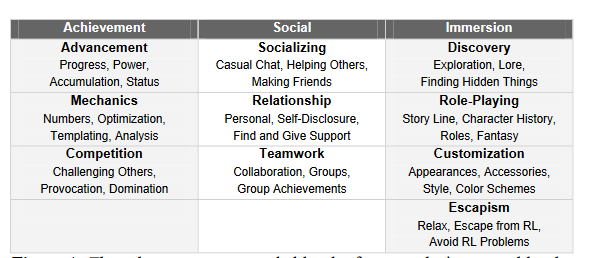
\includegraphics[width=1\linewidth]{content/pictures/nick_yee_categorizations.PNG}
\caption{Motivationsgruppen nach Nick Yee (Quelle: \cite{yee_motivations_nodate})}
\label{fig:nick_yee_motivations}
\end{figure}

Die Achievement-Komponente umfasst den Fortschritt im Spiel sowie das damit einhergehende Verlangen Macht zu erlangen, schnell voranzukommen und Symbole für Reichtum oder Status zu erwerben. Zudem besteht ein Interesse daran, die Spielmechanik zu analysieren, die Regeln und Systeme zu verstehen um die Leistung der Spielfigur zu optimieren. Auch ist der Wettbewerb Spielt eine zentrale Rolle: Es besteht der Wunsch, sich mit anderen zu messen und gegen sie anzutreten.

Die soziale Komponente beschreibt das Bedürfnis nach Sozialisierung. Spieler haben Interesse daran, anderen zu helfen und sich mit ihnen zu unterhalten. Daraus entstehen Beziehungen, bei denen der Wunsch besteht, langfristige und bedeutungsvolle Bindungen zu anderen aufzubauen. Teamarbeit ist dabei ebenfalls gewünscht, um gemeinsame Ziele zu erreichen oder sich im Wettbewerb zu behaupten.

Die Immersion-Komponente beschreibt das Entdecken der Spielwelt und das damit verbundene Finden von Objekten sowie das Erlangen von Wissen, das den meisten anderen Spielern unbekannt ist. Rollenspiel-Elemente sind besonders wichtig, um den Spielfiguren Hintergrundgeschichten zu geben und gemeinsam improvisierte Erzählungen zu entwickeln. Der Spielavatar sollte zudem anpassbar sein, damit persönliche Vorlieben und individueller Stil der Spieler zum Ausdruck kommen können. Die Spielwelt dient auch als Mittel um den Alltag zu entfliehen und den Problemen der realen Welt zu entkommen.

\paragraph{weitere Modelle}
Im Zuge der fortschreitenden Forschungen entstanden weitere Modelle wie zum Beispiel das Gamer Motivation Model, das auf Basis der Forschung von Nick Yee entwickelt wurde (vgl. \cite{ludologie_spielertypen_nodate}):

\begin{figure}[ht]
\centering
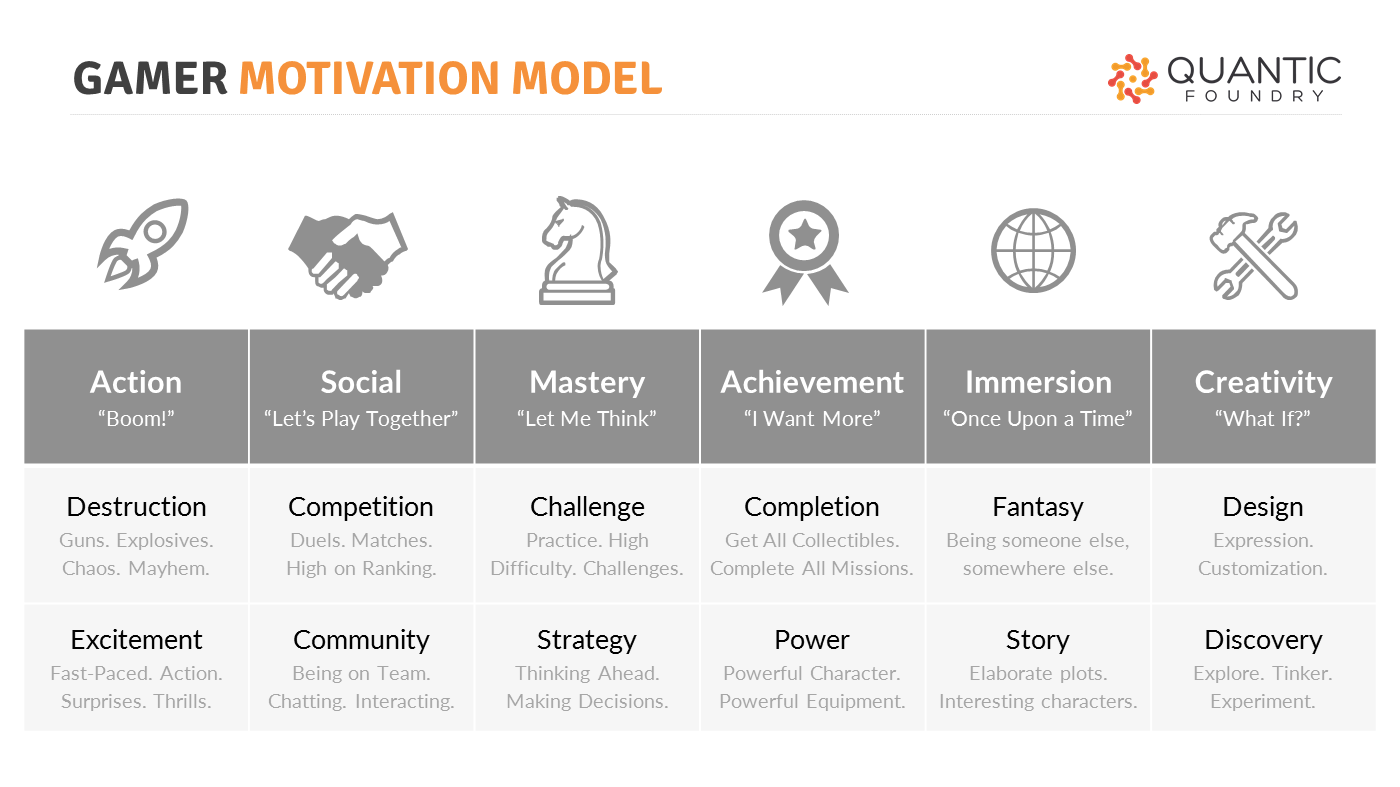
\includegraphics[width=1\linewidth]{content/pictures/gamer_motivations_model.png}
\caption{Gamer Motivation Model der QUANTIC FOUNDRY (Quelle: \cite{noauthor_quantic_nodate})}
\label{fig:gamer_motivation_model}
\end{figure}

Ein weiteres Modell, das in der Arbeit von Bateman genannt wird, ist das BRAINHEX-Model, bei dem die verschiedenen Spielertypen in hexagonaler Anordnung platziert sind (vgl. Abbildung: \ref{fig:brain-hex}):

\begin{figure}[ht]
\centering
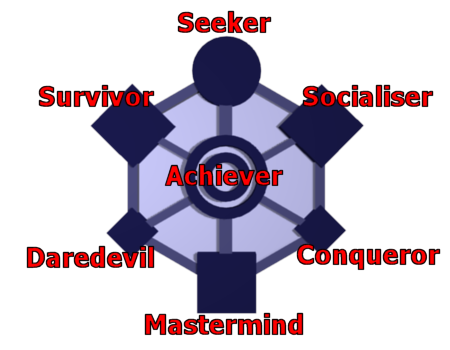
\includegraphics[width=1\linewidth]{content/pictures/brainhex-classes.png}
\caption{Brainhex-Model Darstellung von \cite{noauthor_i_nodate} nach \cite{nacke_brainhex_2013}}
\label{fig:brain-hex}
\end{figure}

% \cite{bartle_hearts_nodate}

% [erwähnen wurde aber rausgelassen, man kann erwähnen, dass es noch weitere klassifizierungen gibt
% \subsection{Das BrainHex-Model}
% \cite{nacke_brainhex_2014}
% ]

% [kommt zu wichtige Begriffe
% \section{Kooperative Gamedesign Pattern}
% \subsection{Was sind Game Pattern}
% \cite{bjork_patterns_2005}

% \subsection{Complementarity}

% \subsection{Synergies}

% \subsection{Abilities}

% \subsection{Shared Goals}

% \subsection{Synergies between goals}

% \subsection{Special Rules for Player of the same Team}

% \subsection{Camera Setting}

% \subsection{Interacting with the same object}

% \subsection{Shared puzzle}

% \subsection{Shared characters}

% \subsection{Special characters targetting lone wolf}

% \subsection{Vocalization}

% \subsection{Limited ressources}

% \subsection{Einflussnahme}
% \cite{emmerich_impact_2017}

% ]
\section{Multiplayer-Spiele}
Im Vergleich zu Einzelspieler-Spielen existieren bei Multiplayer-Spielen nicht nur Unterschiede im Genre, sondern auch in den Spielrollen (Symmetrie / Asymmetrie) sowie in den Spielzeitpunkten, zu denen die Spielteilnehmer an ihrem Spielfortschritt weiterarbeiten (Synchron / Asynchron). [Hier wäre eine Quelle noch gut]. Auf dem Spielemarkt existieren außerdem Multiplayer-Spiele, die unterschiedliche Medientechniken verwenden. Teilweise dienen diese Medientechniken dazu, Cross-Plattform Funktionalität zu gewährleisten (vgl. \cite{noauthor_baldurs_nodate}), oder sie sind integrale Bestandteil des Gamedesigns (vgl. \cite{noauthor_keep_nodate}).

Da im Kontext von \say{Connecting-Minds} die Spieler zeitgleich in einer Sitzung gemeinsam spielen, wird im Folgenden auf die Symmetrie und Asymmetrie von Computer- und Videospielen eingegangen.

% In den folgenden Kapiteln werden die jeweiligen Eigenschaften der unterschiedlichen Ausprägungen von Multiplayer-Spielen aufgezählt.

% \subsection{Synchrone Multiplayer}
% Synchrone Multiplayer-Spiele sind solche, bei denen die Spieler i. d. R. zum selben Zeitpunkt, bzw. zur selben Zeit gemeinsam miteinander oder gegeneinander Spielen. [Quelle suchen]. Weit verbreitet sind hier vorallem Ego-Shooter wie die \say{Call of Duty}-Reihe, bei denen die Spieler innerhalb einer Sitzung gegeneinander im \say{Einzel} oder als \say{Team} gegeneinander Spielen (vgl. \cite{noauthor_call_nodate}).

% \subsection{Asynchrone Multiplayer}
% Asynchrone Multiplayer-Spiele werden zeitversetzt gespielt. [Quelle und beispiele suchen]

\subsection{Symmetrische Multiplayer}
Symmetrische Spiele sind solche, bei denen alle Spieler die gleichen Spielregeln haben und das gleiche Spielziel verfolgen. Viele traditionelle Spiele wie Schach sowie Computer- und Videospiele wie \say{Mario Kart} oder \say{Minecraft} sind symmetrische Multiplayer-Spiele, bei denen für jeden Spieler das gleiche Ziel gilt (vgl. \cite[S. 12]{adams_fundamentals_2013}); (vgl. \cite{noauthor_mario_nodate}); (vgl. \cite{noauthor_willkommen_nodate}). 


\subsection{Asymmetrische Multiplayer}
Asymmetrische Spiele hingegen können unterschiedlichen Spielern unterschiedliche Regeln zugestehen und verfolgen ebenfalls unterschiedliche Ziele (vgl. \cite[S. 12]{adams_fundamentals_2013}). Sie sind sowohl in kooperativen als auch kompetitiven Spielen weit verbreitet und werden bspw. in Form verschiedener \say{Helden} oder \say{Klassen} umgesetzt. So gibt es z.B. in \say{Overwatch} oder \say{League of Legends}  unterschiedliche \say{Support}-Charaktere, deren Aufgabe es ist das Team zu heilen (vgl. \cite{smilovitch_birdquestvr_2019}); (vgl. \cite{noauthor_league_2025}); (vgl. \cite{noauthor_overwatch_nodate}). 
Außerdem ermöglichen asymmetrische Spiele, dass Spieler mit unterschiedlichen Fähigkeiten und Fähigkeitsniveaus gemeinsam spielen können. Ein asymmetrisches Design kann zudem die Inklusivität in Spielen fördern (vgl. \cite{smilovitch_birdquestvr_2019}).

\subsection{Hybride Multiplayer}
Wie \cite[S. 6f]{lotz_konzeption_2021} in ihrer Bachelor-Arbeit beschrieben hat, unterscheiden sich Multiplayer auch in der verwendeten Medientechnik. Sogenannte hybride Spiele wie \say{New Super Mario Bros U} (vgl. \cite{noauthor_mario_nodate-1}).

\begin{figure}[ht]
\centering
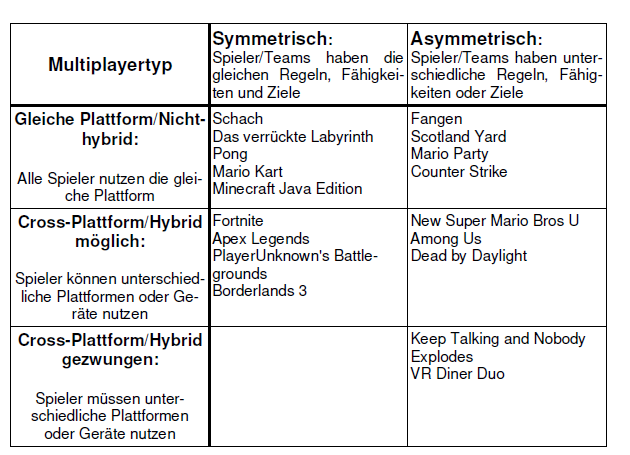
\includegraphics[width=1\linewidth]{content/pictures/lotz_hybrid_multiplayer.PNG}
\caption{Unterscheidung Multiplayertypen (Quelle: \cite[S.6]{lotz_konzeption_2021})}
\label{fig:lotz_multiplayer_types}
\end{figure}

Wie Abbildung \ref{fig:lotz_multiplayer_types} zeigt, können Multiplayer-Spiele hinsichtlich ihrer Medientechnik in drei Kategorien eingeteilt werden.
Spiele wie \say{Mario Kart} oder \say{Minecraft} können nur auf der gleiche Plattform gespielt werden. Bei Spielen wie \say{Among Us} oder \say{Fortnite} ist die Plattform, auf der gespielt wird, nicht relevant, da eine Cross-Play-Funktionalität gegeben ist. Jeder kann mit Spielern auf der Plattform spielen, die er zu zuhause hat. Die dritte Kategorie umfasst Spiele, bei denen die Spieler gezwungen werden, unterschiedliche Plattformen zu nutzen. In \say{Keep talking and nobody explodes} ist dies der Kern des Gamedesigns.

\section{Spielweisen von Multiplayer-Spielen}
Nachdem die unterschiedlichen Strukturen und technischen Formen von Multiplayer-Spielen behandelt wurden, ist es nun wichtig, die verschiedenen Spielweisen zu betrachten. Multiplayer-Spiele können dabei in drei Hauptspielformen unterteilen:
auf kompetitive, kollaborative und kooperative Spielweisen. [Quelle finden]

\subsection{Kompetitiv}
Kompetitive Spiele sind solche, bei denen Spieler oder Teams gegeneinander antreten, um ein bestimmtes Ziel zu erreichen, wobei der Erfolg des einen oft den Misserfolg des anderen bedeutet. In diesen Spielen ist das Spiel selbst neutral und agiert nicht aktiv im Wettbewerb (vgl. \cite{noauthor_game_2014}). [noch andere Quellen suchen]

\subsection{Kollaborativ}
Kollaborative Spiele sind solche, bei denen alle Spieler - ähnlich wie in Kooperationsspielen - gemeinsam gegen das Spiel verlieren können. Allerdings können sie nicht gemeinsam gewinnen. Diese Spiele sind im Kern meist kompetitiv, beeinhalten jedoch die Möglichkeit einer kollektiven Niederlage. Die Spieler müssen zu einem gewissen Maß zusammenarbeiten, um nicht zu verlieren (vgl. \cite{noauthor_game_2014}). [noch andere Quellen suchen]

\subsection{Kooperativ}
Bei Kooperationsspielen ist es möglich, dass alle Spieler gemeinsam gegen das Spiel verlieren oder gemeinsam gewinnen können. Ein Sieg wird erreicht, wenn das Spiel gemeinsam \say{besiegt} wird oder dadurch dass ein festgelegtes Ziel kollektiv oder individuell erreicht werden kann (vgl. \cite{noauthor_game_2014}). [noch andere Quellen suchen]

% \section{Artverwandte Spiele}
% Nachdem nun die einzelnen Charakteristiken von Multiplayer-Spielen aufgezeigt wurden, werden nun Spiele vorgestellt, welche im Rahmen dieser Arbeit näher betrachtet wurden.

% Die Spielreihe \say{\textbf{We were here}} vom niederländischen Entwicklerstudio Total Mayhem Games beinhaltet asymmetrische Kooperative-Multiplayer-Spiele, bei denen zu zweit Rätsel und Hindernisse in der Spielwelt gelöst werden müssen um aus der Umgebung, in denen die Avatare der Spieler gefangen sind, zu entkommen. Dabei können die Spieler über ein \say{In-Game}-Walki-Talki miteinander kommunizieren. Zumeist ist es so, dass ein Spieler verschiedene Rätsel oder Hindernisse für sich hat, die er seinem Mitspieler beschreiben muss, damit dieser die passenden Antworten übermitteln oder Rätsel lösen kann. Die beiden Spieler befinden sich dabei in abgetrennten Räumen oder Gebieten innerhalb der Spielwelt (vgl. \cite{noauthor_we_nodate}; \cite{noauthor_total_nodate}).  

% [hier it takes two und split fiction erwähnen]

% Das Spiel \say{\textbf{The past within}} vom ebenfalls aus den Niederlanden kommenden Entwicklerstudio Rusty Lake ist ein asymmetrisches kooperatives Multiplayer-Spiel bei dem zwei Spieler gemeinsam in einer Sitzung sowohl in der Vergangenheit als auch in der Zukunft gemeinsam Rätsel lösen müssen um der Protagonistin und ihrem Vater zu helfen. Jeweils ein Spieler befindet sich dabei in einer 2D-Amnwendung, der andere in einer 3D-Anwendung. Es existiert die Möglichkeit, dass das Spiel von verschiedenen Plattformen aus gespielt werden kann (Cross-Plattform Spielbarkeit) (vgl. \cite{noauthor_past_nodate}). 

% Das bereits in den vorangegangenen Kapiteln [Kapitel einbinden] erwähnte \say{\textbf{Keep Talking and Nobody Explodes}} ist ein asymmetrisches kooperatives Multiplayer-Spiel bei dem eine Person das Spiel besitzen muss damit es im Team gespielt werden kann. Das Spiel hat eine Besonderheit, da es ein Cross-Plattform Spiel ist, bei dem ein Teilnehmer (der Bombenentschärfer) eine Bombe entschärfen muss und die anderen Spielteilnehmer (die Experten) verschiedene Anleitungen von Bomben vorliegen haben. Die Aufgabe besteht darin die richtige Anleitung für die entsprechende Bombe zu finden und die Bombe innerhalb der vorgegebenen Zeit zu entschärfen. Im Spiel befindet sich jedoch nur der Bombenentschärfer, während die Experten die Anleitungen ausgedruckt durchschauen können (vgl. \cite{noauthor_keep_nodate}).

% Im März 2025 erschien das Spiel \say{\textbf{Myrmidon}} vom Studio Studio Popot, welches ein asymmetrischer kooperativer Multiplayer ist, bei dem zwei Spieler zusammen, in zwei verschiedenen Rollen, miteinander spielen können. Eine Rolle ist dabei die Stop-Motion Puppe, welche in einer Stop-Motion Welt Hindernisse überqueren und über verschiedene Plattformen springen muss um ans Ziel zu kommen. Unterstützt wird die Puppe dabei vom Animator, der die Kulisse des Stop-Motion Films bedienen muss, damit die Puppe an ihr Ziel gelangt (vgl. \cite{noauthor_myrmidon_2024}).

\section{Augmented Reality}

\section{Netzwerkinfrastrukturen}\label{sec:basics-network-structures}
Um ein Multiplayer-Spiel entwickeln zu können, muss zunächst geklärt werden, wie die Netzwerkinfrastruktur der Anwendung aufgebaut sein soll. Es existieren zahlreiche Ansätze, die jeweils für verschiedene Anwendungszwecke konzipiert sind.

\subsection{Distributed Authority}
Bei einer \say{Distributed Authority}-Netzwerktopologie übernimmt jeder im Netzwerk verbundene Spielclient gemeinsam jeweils die Verantwortung für das Erstellen und Verwalten von Objekten im Netzwerk. Jeder Client simuliert dabei seinen Teil der Spielwelt selbst und steuert Objekte über die er Autorität besitzt.
Damit Positionen und andere relevanten Daten an alle anderen Clients im Netzwerk weitergeleitet werden können,wird ein zentraler, leichtgewichtiger Statusdienst verwendet, der ausschließlich für die Verteilung der notwendigen Informationen zuständig ist, ohne selbst die Anwendung zu simulieren (vgl. \cite{noauthor_distributed_2025}).

\begin{figure}[ht]
\centering
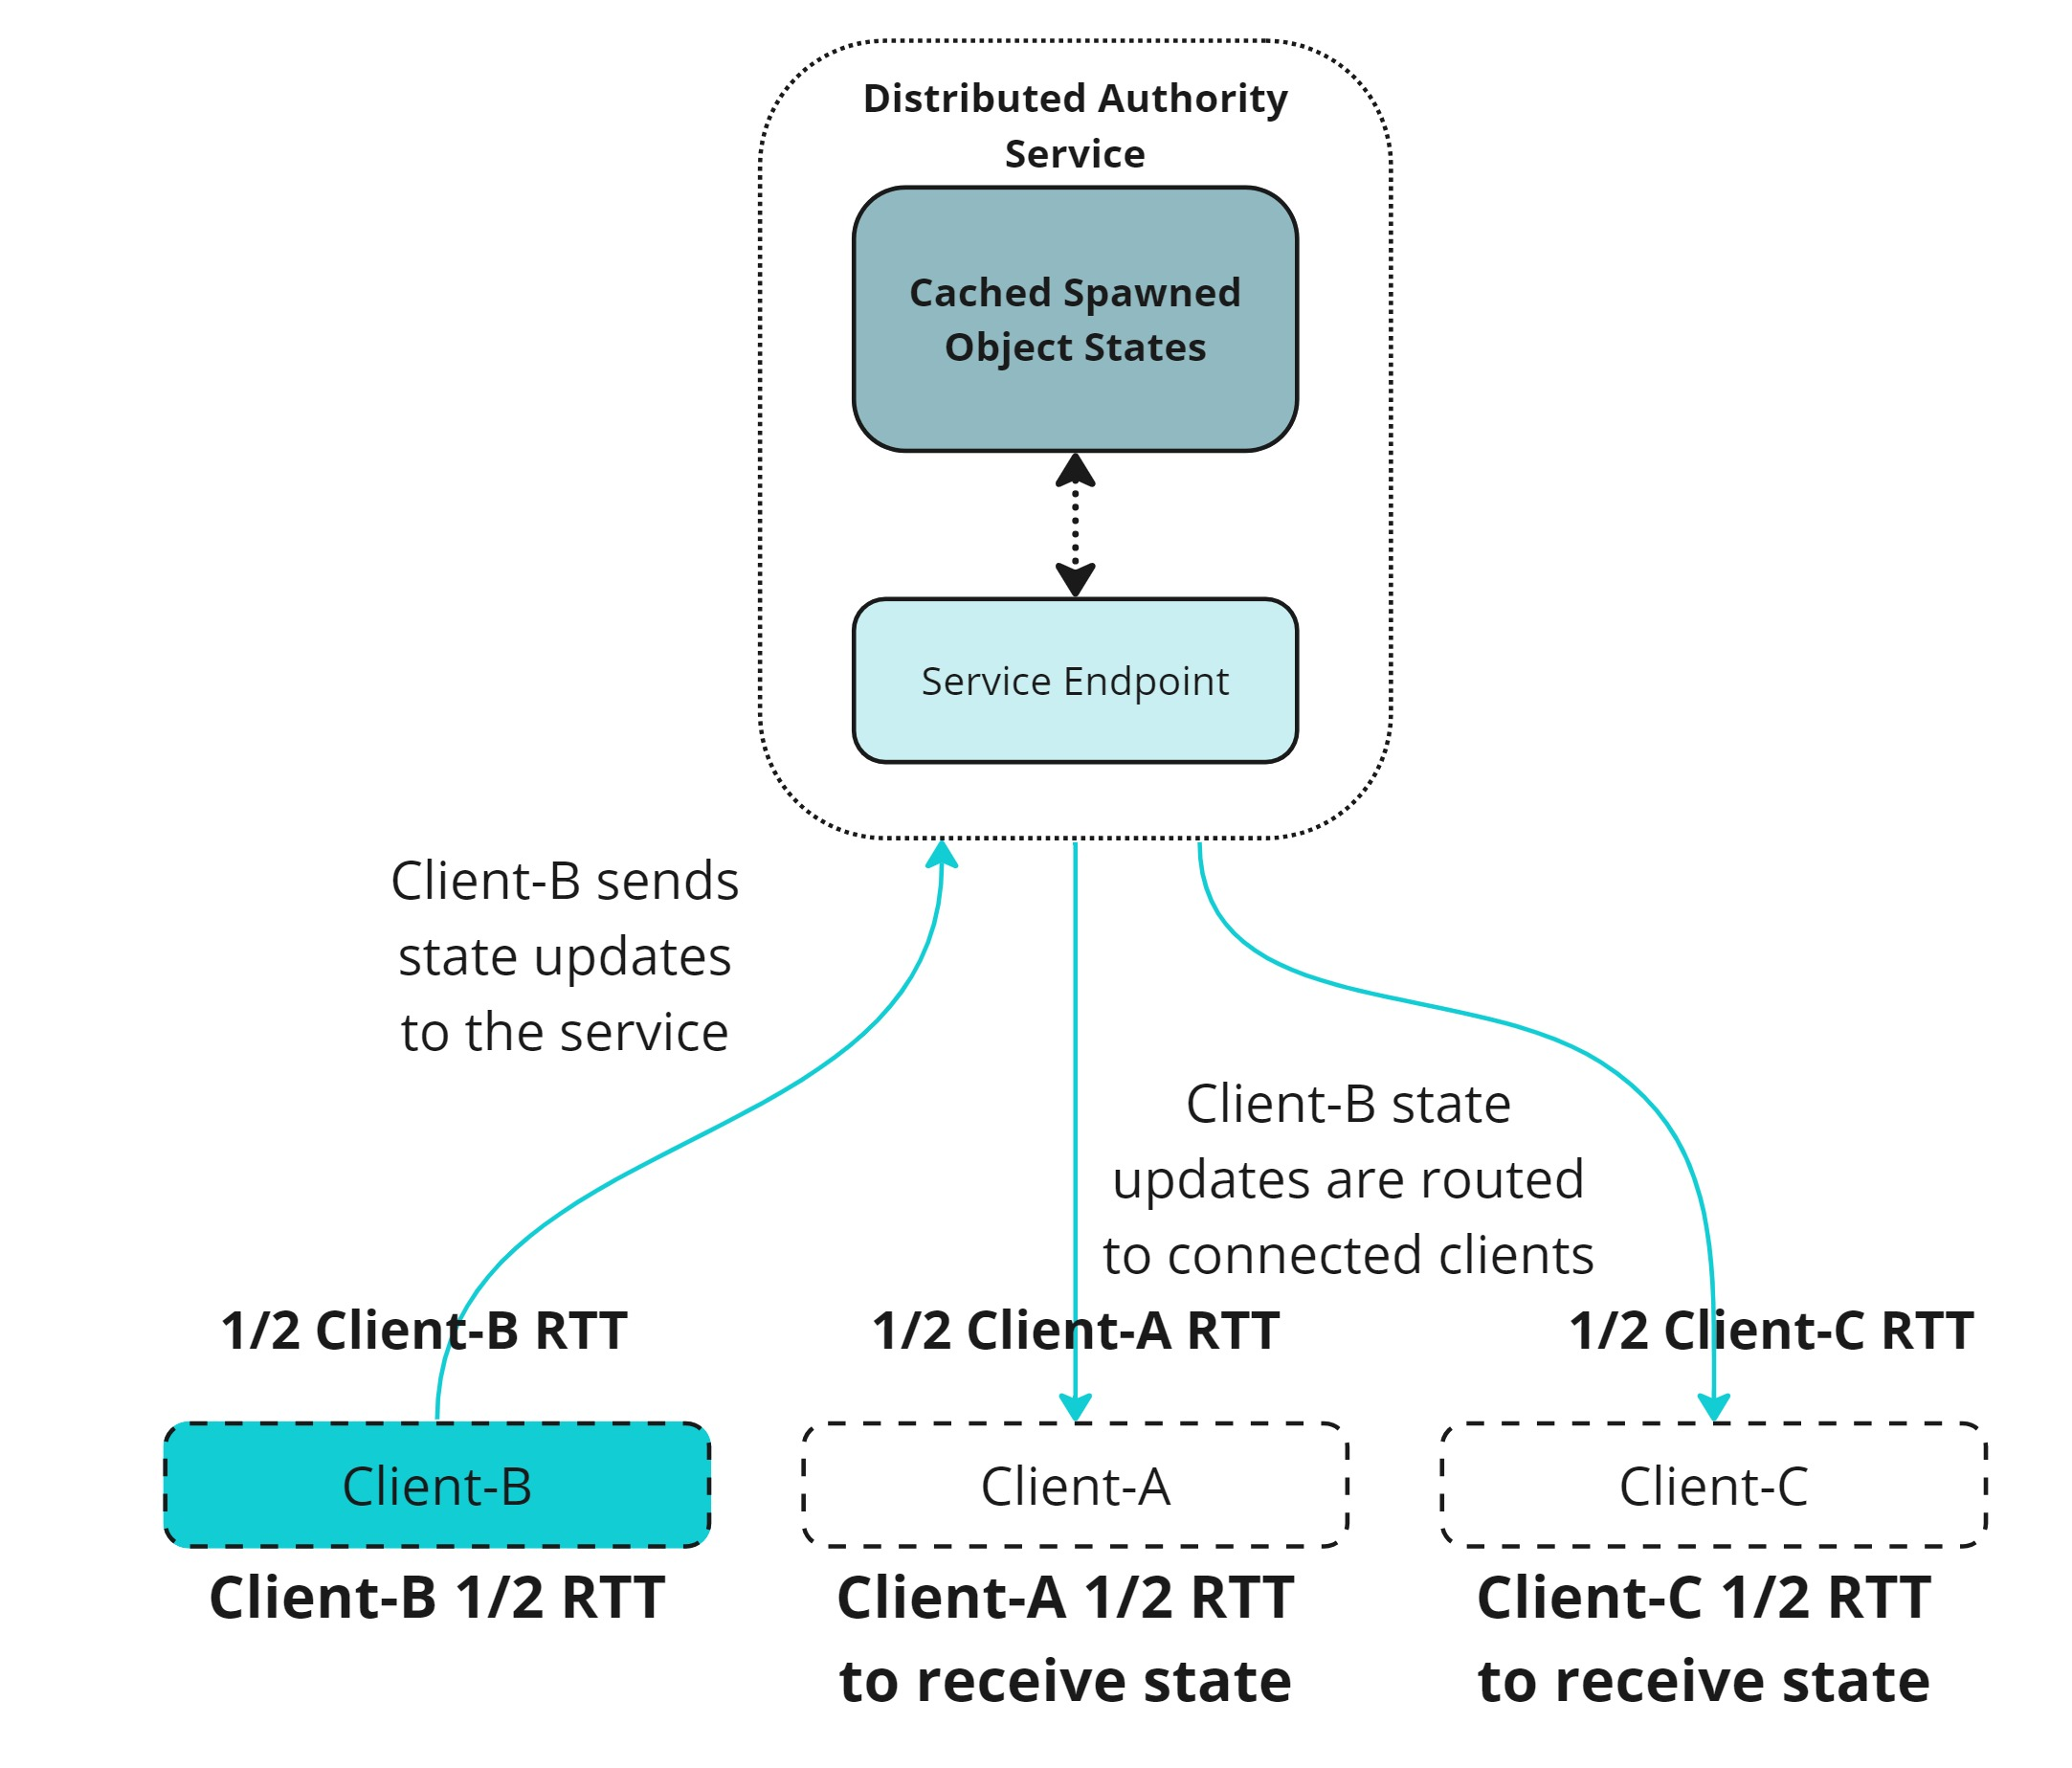
\includegraphics[width=1\linewidth]{content/pictures/distributed-authority-service.jpg}
\caption{Netzwerktopologie der Distributed Authority (Quelle: \cite{noauthor_distributed_2025})}
\label{fig:distributed_authority_topology}
\end{figure}

Spiele wie \say{Journey}, \say{God of War: Ascension}, \say{Mercenaries 2}, \say{GTA: Online}, \say{Dark Souls} und \say{Destiny} nutzen diese Netzwerkinfrastruktur. Häufig kommt diese Topologie zum Einsatz, wenn ein bestehendes Single-Player um eine Multiplayer-Komponente erweitert werden soll (Journey, GTA und Dark Souls), ohne den Kern des Quellcodes grundlegend umzustrukturieren. Diese Architektur erfordert keinen dedizierten Server, eignet sich für Spiele mit großen, offenen Spielwelten (Dark Souls, GTA) und kommt häufig zum Einsatz, wenn keine deterministische Physik benötigt wird bzw. kein vollständig deterministisches Spielkonzept vorliegt. Sie eignet sich zudem besonders für Spiele, bei denen die Prozessorleistung (z.B. durch Physiksimulationen= stark beansprucht wird. Für Spiele mit kooperativen Spielmechaniken, leichten kompetitiven Elementen oder innovativen Multiplayer-Ideen ist diese Infrastruktur eine sinnvolle Wahl (vgl. \cite{noauthor_choosing_2024}).

\subsection{Pure Client/Server}
Bei der Client-Server-Architektur übernimmt ein zentraler Server die Hauptsimulation und verwaltet alle wesentlichen Aspekte des Spiels. Dazu gehören unter anderem die Physiksimulation, das Erzeugen und Entfernen von Objekten sowie die Autorisierung von Anfragen der Clients. Aus Sicht der Clients besitzen diese lediglich die Anwendung, über die sie sich mit dem Server verbinden, und erhalten über diese Verbindung die Darstellung des Spiels (vgl. \cite{noauthor_client-server_2024}):
\paragraph{Ein dedizierter Server} bildet eine eigenständige Instanz, die ausschließlich dem Spielbetrieb dient (vgl. Abbildung \ref{fig:dedicated_server}).

\begin{figure}[ht]
\centering
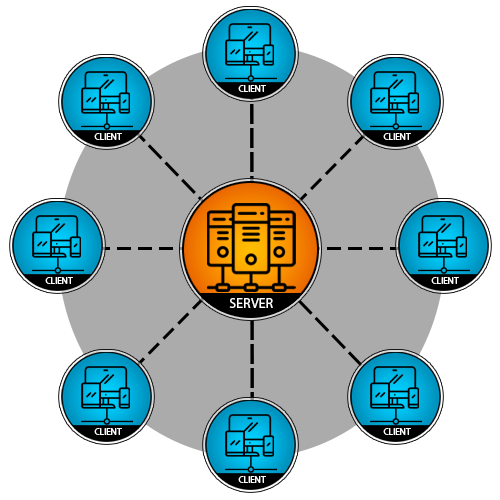
\includegraphics[width=1\linewidth]{content/pictures/ded_server-d5369721966357b9b4d5e1fa96b05b22.png}
\caption{Client-Server-Architektur mit dediziertem Server (Quelle: \cite{noauthor_network_2024})}
\label{fig:dedicated_server}
\end{figure}

\paragraph{Ein Client gehosteter Server} läuft auf demselben Gerät wie die dazugehörige Client-Anwendung (vgl. Abbildung \ref{fig:client_server}).

\begin{figure}[ht]
\centering
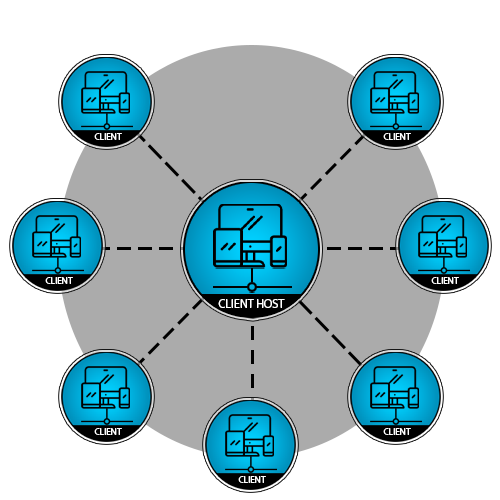
\includegraphics[width=1\linewidth]{content/pictures/client-hosted-16be0b1c9b5020f21325b1e6a7beca73.png}
\caption{Client hosted Server (Quelle: \cite{noauthor_network_2024})}
\label{fig:client_server}
\end{figure}

% \subsection{Client-Side Prediction and Lag Compensation}

% Spiele wie \say{Counterstrike}, \say{Call of Duty}, \say{Valorant} und \say{Apex legends} verwenden ein auf dem klassischen Quake-Modell basierendem Netzwerkmodell. Der Spieler steuert dabei lokal im eigenen Client, auf dem die volle Simulation läuft, ohne dabei Verzögerungen beim Laufen oder Schießen zu haben. Der Server nimmt die Eingaben samt Zeitstempel des Clients entgegen und verteilt den \say{State} zurück. Bspw. das Inventar, Munition oder Feuerraten. Die Korrekturen des \say{State}s werden rückwirkend auf den Client angewandt, der den Zustand bis zur aktuellen Zeit wieder herstellt (\say{Client-Side Prediction}). Schüsse und der damit einhergehende Schaden wir auf dem Server ausgewertet und an die Clients übergeben. Um das Spielerlebnis reaktionsschnell und präzise zu gestatlten, nutzt der Server ein \say{Lag Compensation} Verfahren, bei dem er anhand gespeicherter Zustände die Welt aus der Sicht der Clients zum Schlusspunkt rekonstruiert wird (vgl. \say{}.

\subsection{Peer-to-Peer}
Das \ac{P2P}-Architektur-Modell verbindet jeden Spieler direkt mit allen anderen.Über diese Verbindungen werden Daten zu Spielzuständen und Ereignissen ausgetauscht. Im \say{reinen} \ac{P2P}-System gibt es keinen zentralen \say{Host}. Stattdessen ist jeder Client dafür verantwortlich, seinen eigenen Avatar (oder seine Einheiten) zu verwalten und erhält gleichzeitig Updates von den anderen Clients (vgl. \cite{mygames_unity_2024}). Abbildung \ref{fig:p-2-p} zeigt die entsprechende Topologie.

\begin{figure}[ht]
\centering
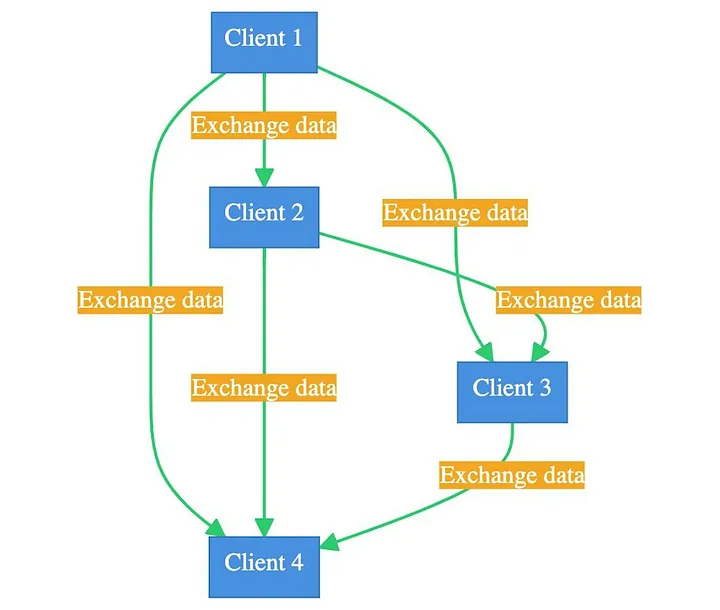
\includegraphics[width=1\linewidth]{content/pictures/0_poGQC2fWQ3tPWPwT.png}
\caption{Peer-to-Peer Infrastruktur (Quelle: \cite{mygames_unity_2024})}
\label{fig:p-2-p}
\end{figure}


\subsection{Relay-Server}
Der Relay-Dienst ermöglicht Multiplayer-Unterstützung ohne die Notwenigkeit eines dedizierten Spielserver. Dabei wird die Kommunikation die Kommunikation zwischen den Spielern über sogenannte Relay-Server weitergeleitet. Nachrichten werden mithilfe einer latenzarmen Datagramm-Übertragung übermittelt, sodass keine direkte Verbindung zwischen den einzelnen Spielern erforderlich ist (vgl. \cite{noauthor_relay_nodate}).

\begin{figure}[ht]
\centering
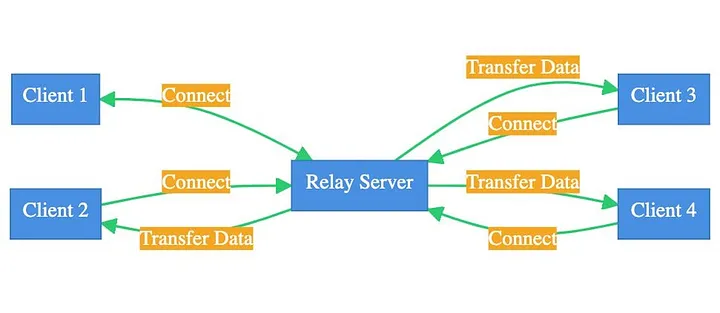
\includegraphics[width=1\linewidth]{content/pictures/0_o7LJU1ImxPHIM5Ej.png}
\caption{Relay-Server Infrastruktur (Quelle: \cite{mygames_unity_2024})}
\label{fig:relay-server}
\end{figure}

% \subsection{Verwendete Kommunikationsprotokolle}
% [überlegung hier noch die protokolle erwähnen]

